% !TEX root = ../main.tex
\backupbegin
%---------------------------------------------------------------------------------------------------
%---------------------------------------------------------------------------------------------------
\subsection{Appendix}

%---------------------------------------------------------------------------------------------------
%---------------------------------------------------------------------------------------------------
\begin{frame}{Data and estimation}\vspace{0.25cm}

	\heading{Dataset}\vspace{-0.75cm}
	\begin{align*}
		\mathcal{D} = \{a_{it}, \bar{s}_{it}, \bar{u}_{it}: i = 1, \hdots, N; t = 1, \hdots, T_i\}
	\end{align*}

\vspace{0.3cm}
\begin{multicols}{2}

	\heading{State variables}\vspace{0.25cm}
	\begin{itemize}\setlength\itemsep{1em}
	\item $s_t = (\bar{s}_t, \epsilon_t)$\medskip
	\begin{itemize}\setlength\itemsep{1em}
		\item $\bar{s}_t$ observed
		\item $\epsilon_t$ unobserved
	\end{itemize}
	\end{itemize}

\columnbreak

\pause

\heading{Likelihood-based estimation}\vspace{-0.95cm}

\begin{align*}
	  \hat{\btheta} = \argmax_{\btheta \in \bTheta} \prod^N_{i= 1} \prod^{T_i}_{t= 1}\, p_{it}(a_{it}, \bar{u}_{it} \mid \bar{s}_{it}, \btheta)
	\end{align*}

\end{multicols}

\label{Data and estimation}
\hyperlink{fig-model-fit}{\beamerbutton{Explore model fit}}

\end{frame}
%---------------------------------------------------------------------------------------------------
%---------------------------------------------------------------------------------------------------
\begin{frame}\label{fig:final-school}
    \setcounter{subfigure}{0}
    \begin{figure}[h!]\centering
    \subfloat[Type 1]{\scalebox{0.25}{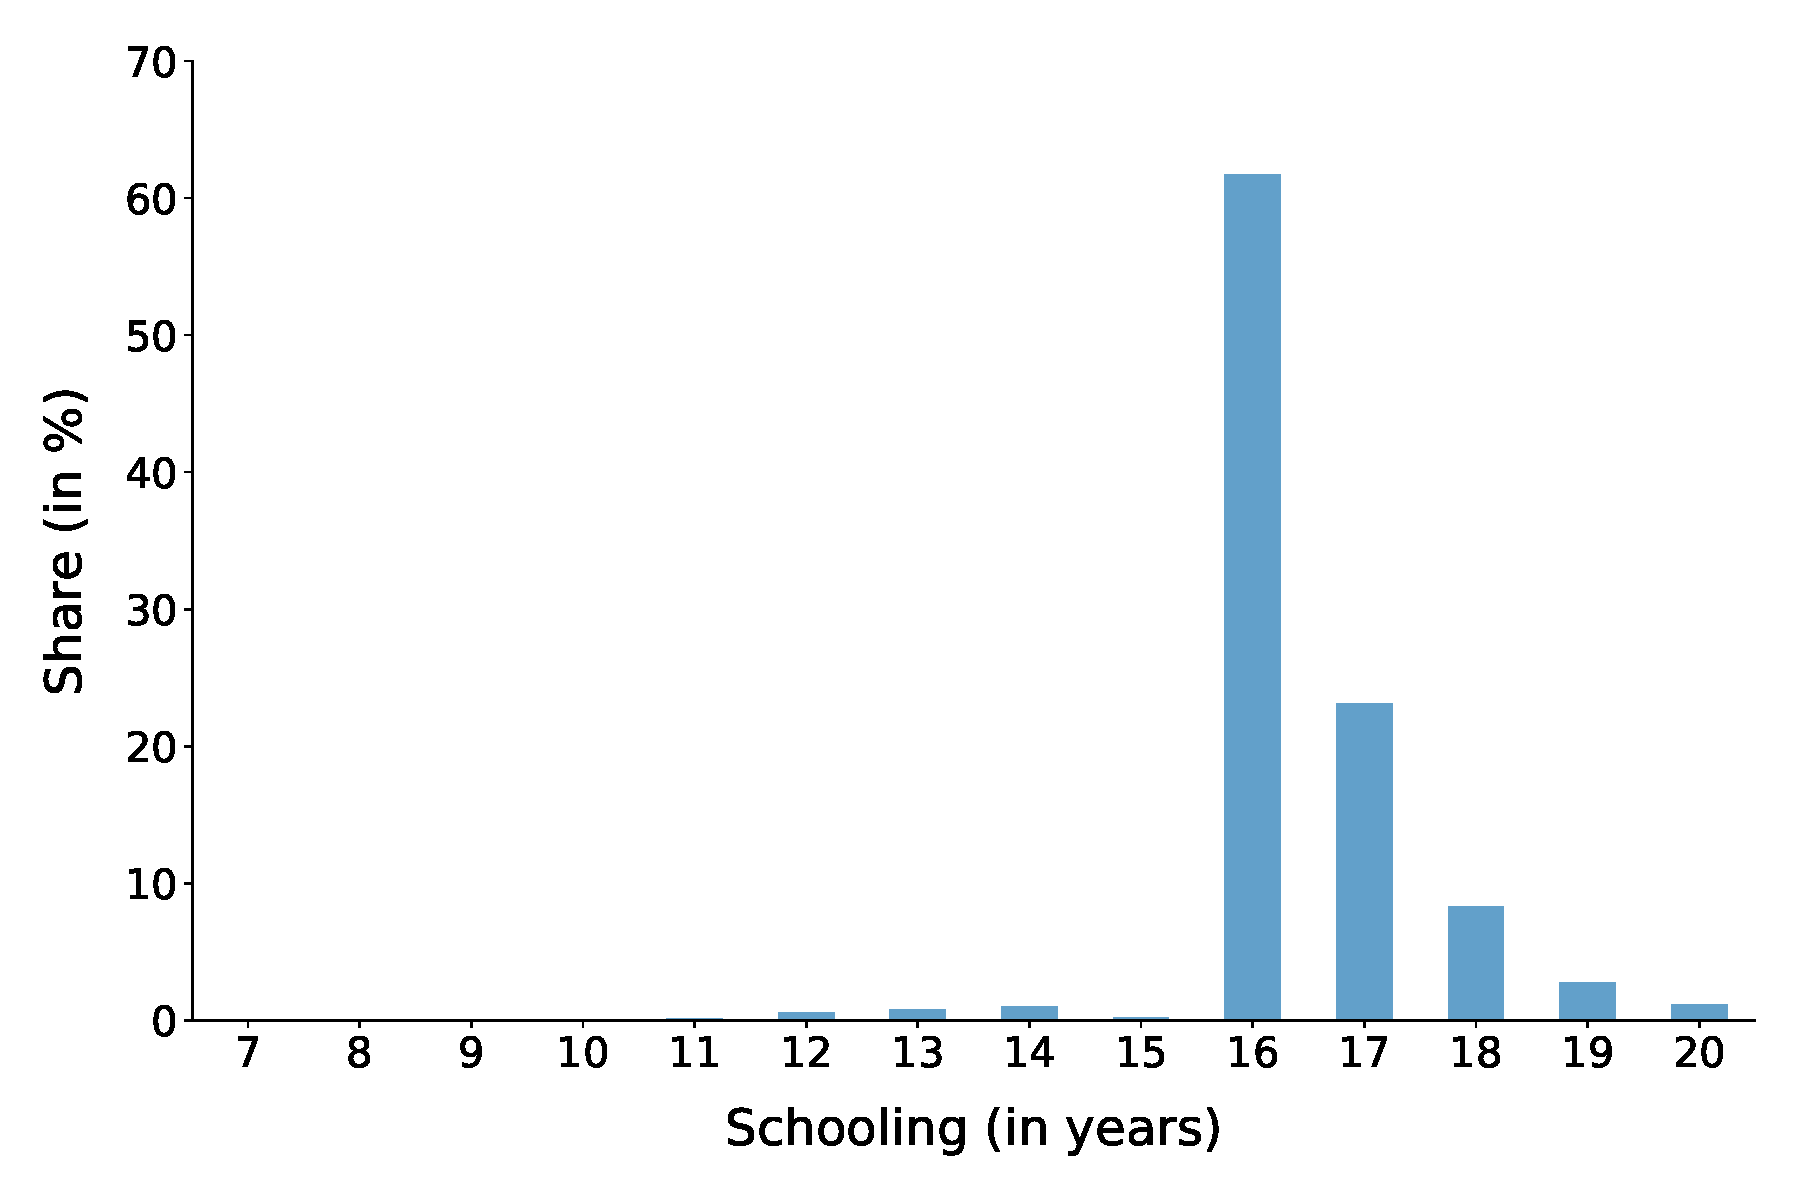
\includegraphics{fig-data-final-schooling-type-0}}\label{type 0}}
    \subfloat[Type 3]{\scalebox{0.25}{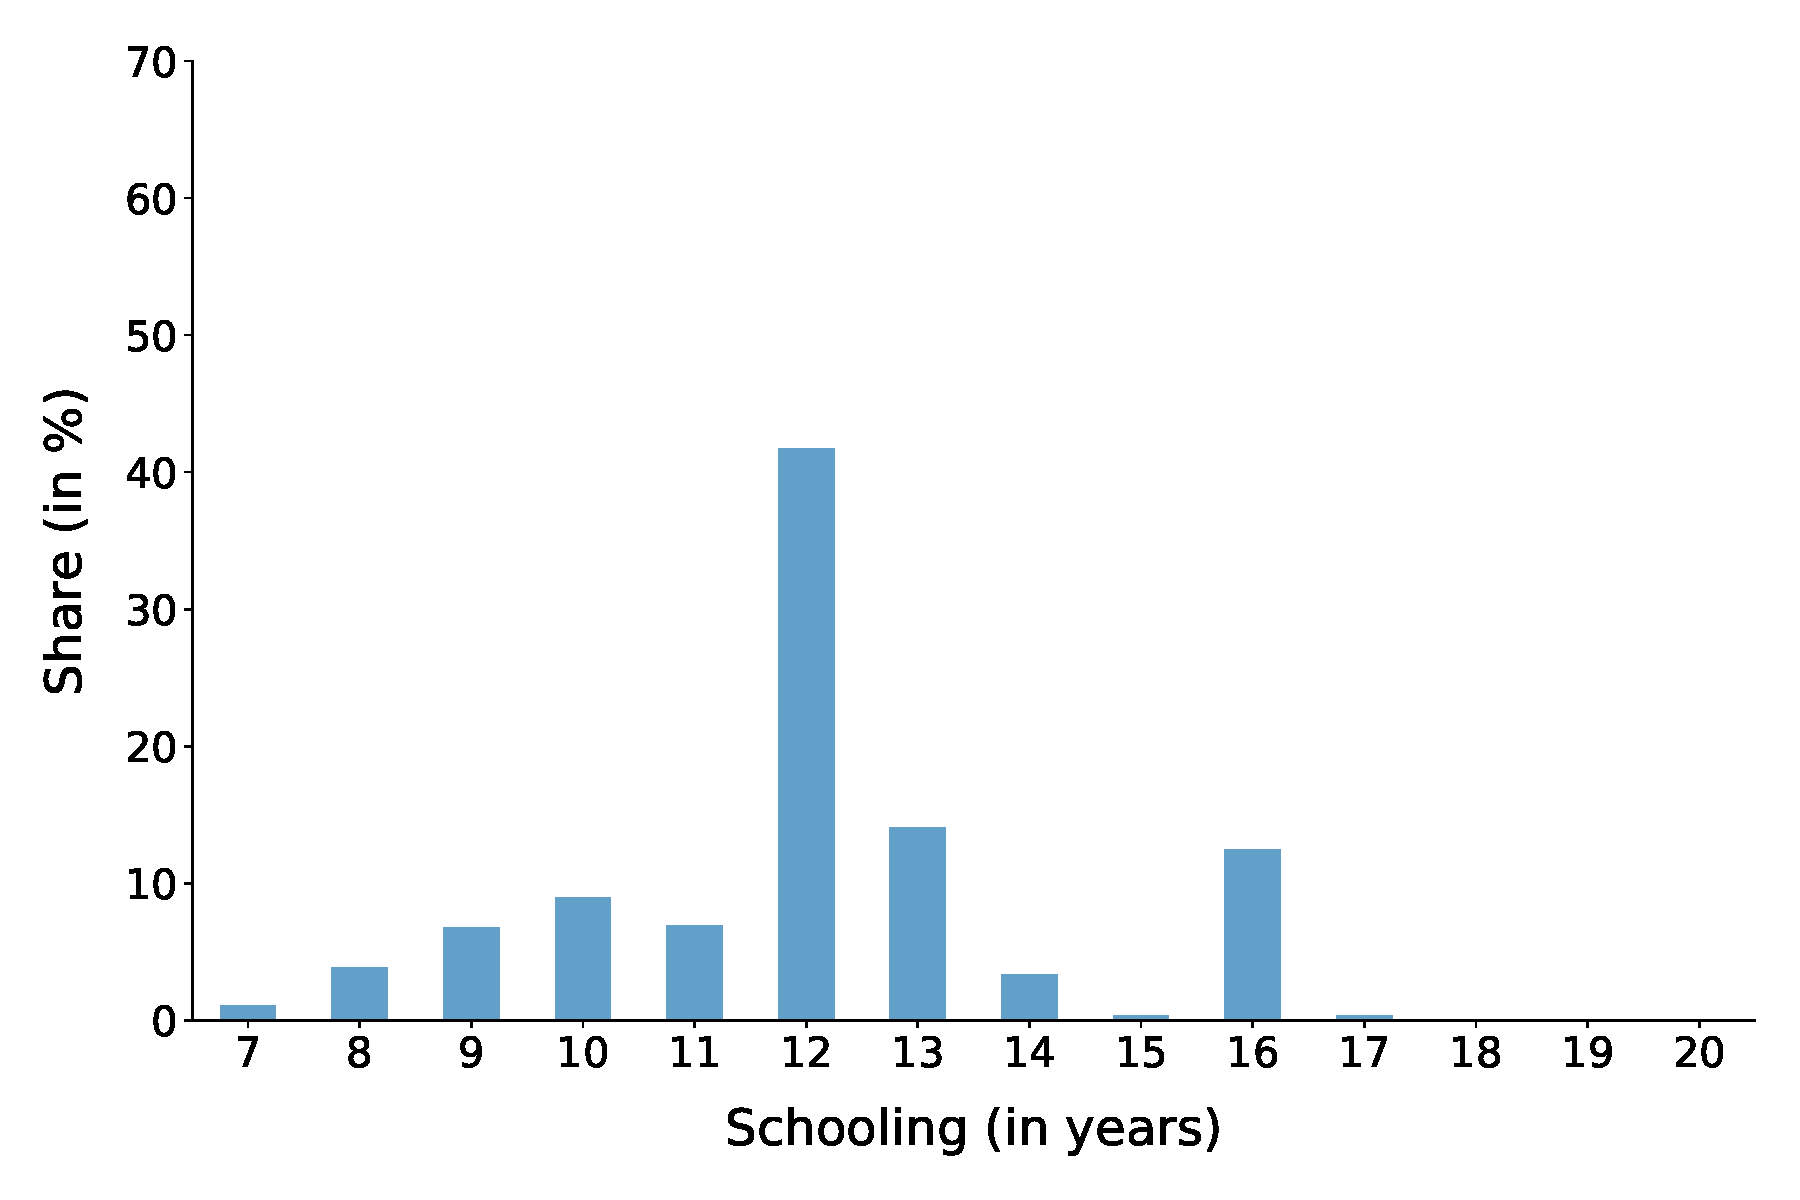
\includegraphics{fig-data-final-schooling-type-2}}\label{type 2}}
    \caption{Final distribution of schooling}\label{Targeted subsidy}
    \end{figure}
    {\vspace{-25pt} \hyperlink{fig:targeting-policies}{\beamerbutton{Heterogeneity in uncertainty}}}
\end{frame}
%---------------------------------------------------------------------------------------------------
%---------------------------------------------------------------------------------------------------
\begin{frame}\label{fig:final-school-policy}
  \begin{figure}[h!]\centering
  \subfloat[Low $\delta$]{\scalebox{0.25}{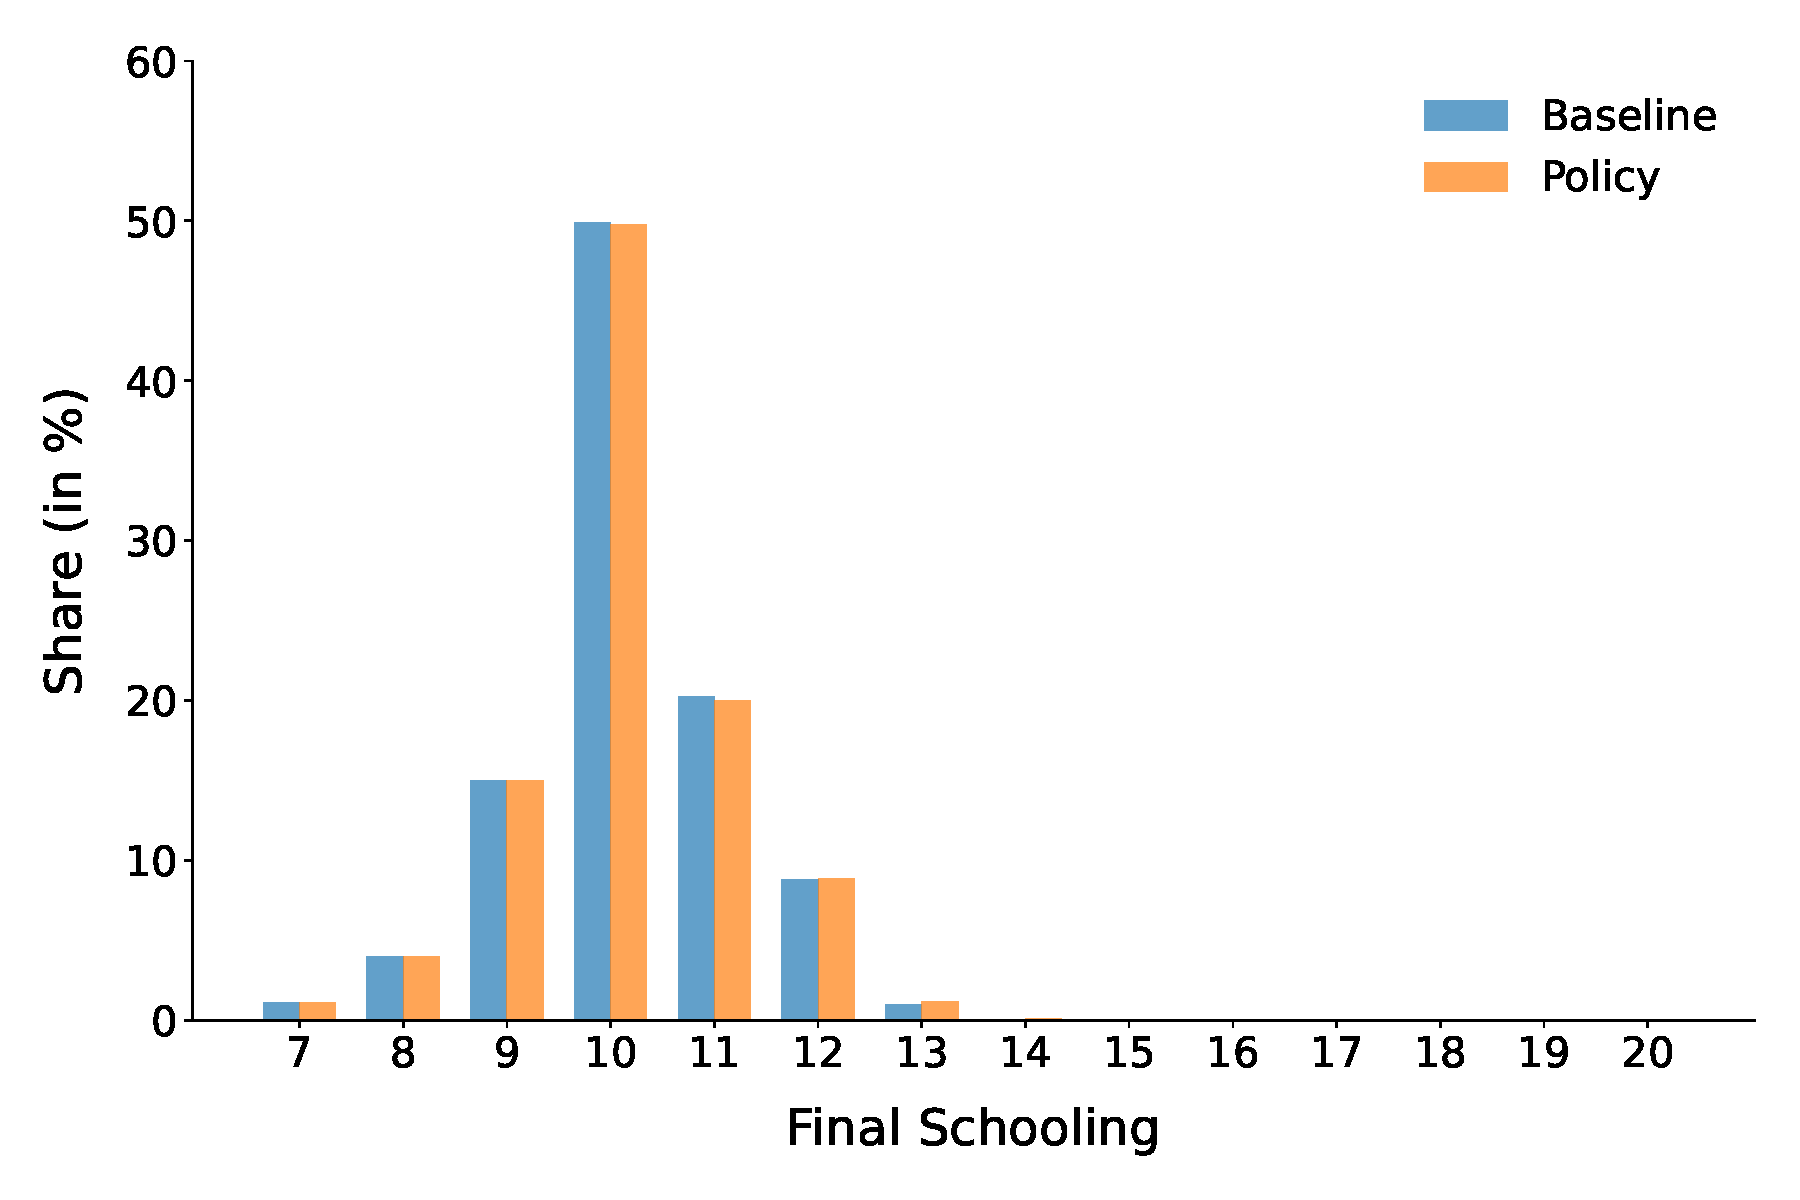
\includegraphics{fig-policy-impact-delta-low}}}
  \subfloat[High $\delta$]{\scalebox{0.25}{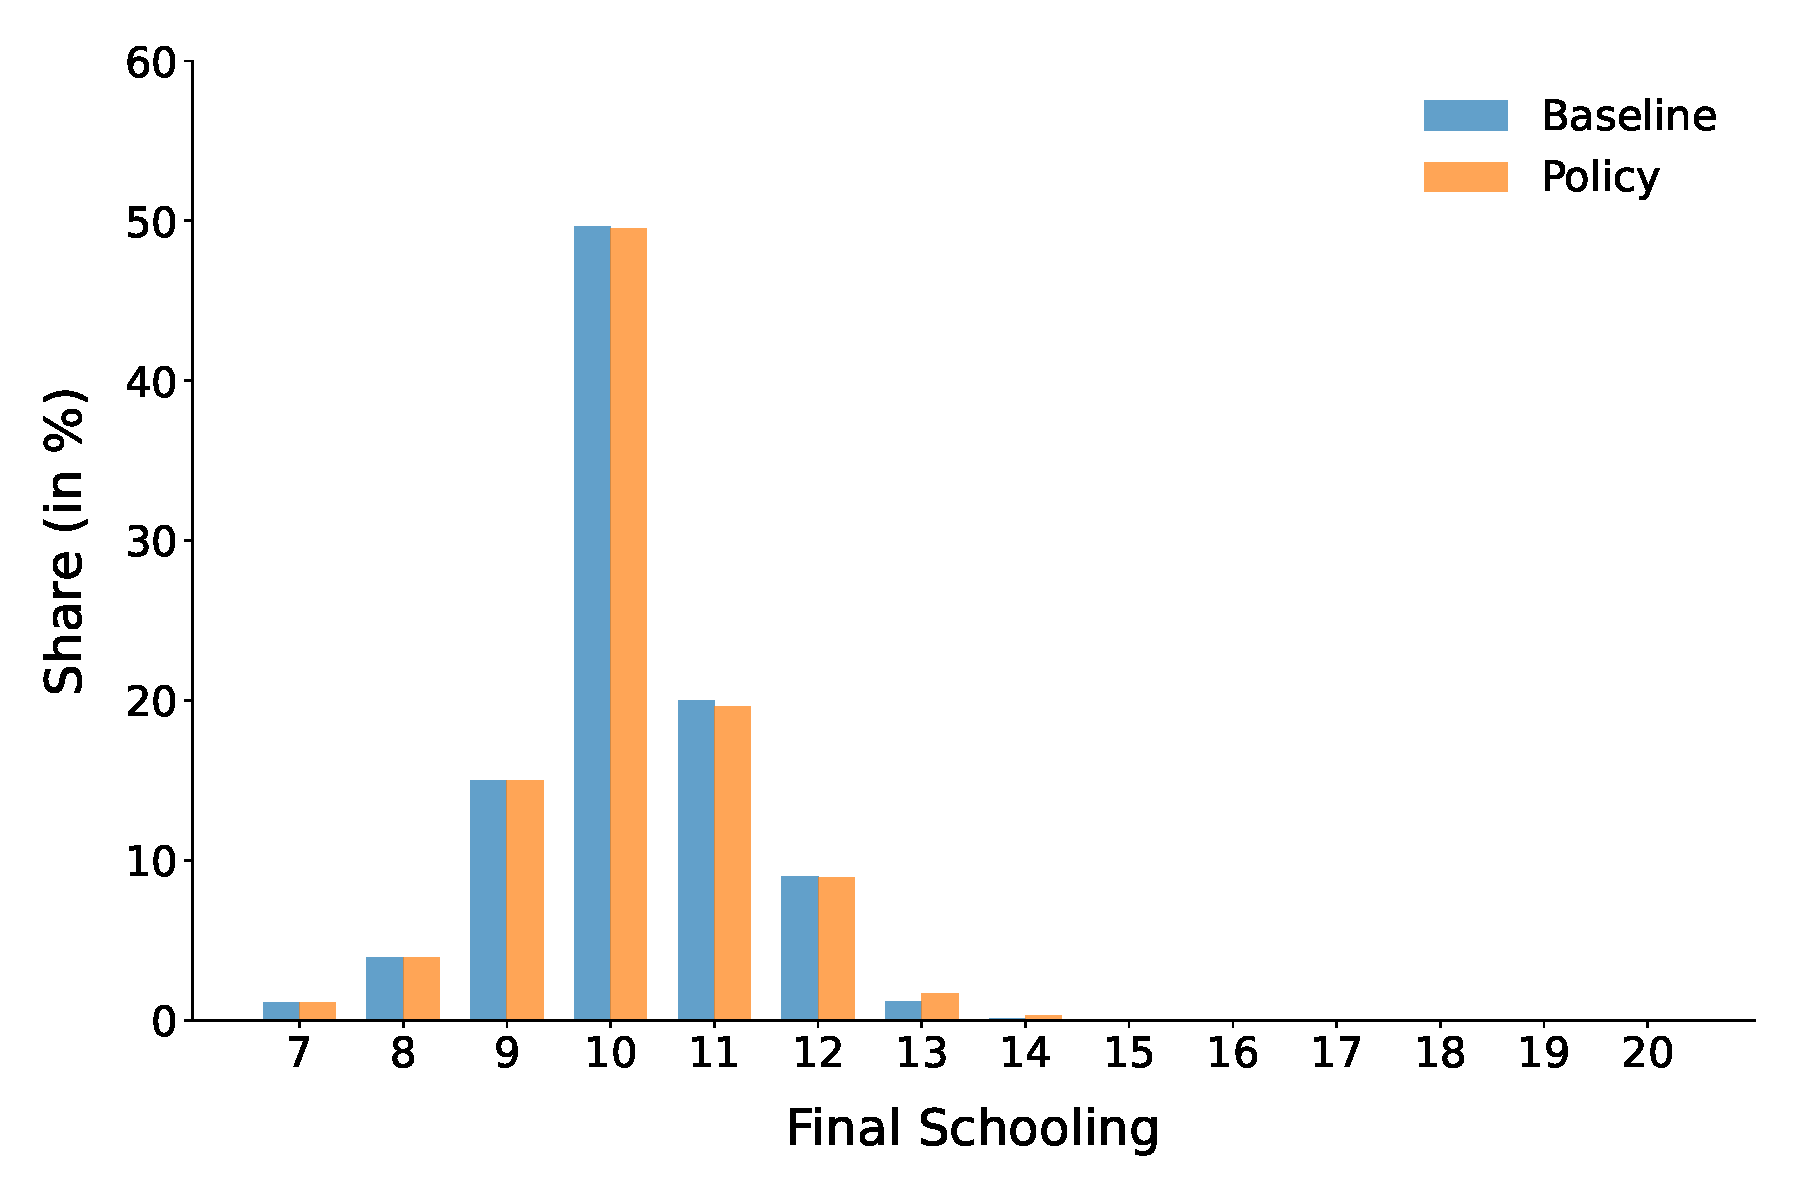
\includegraphics{fig-policy-impact-delta-high}}}
  \caption{Policy impact and time preference}\label{Policy impact and time preference}
  \end{figure}
    {\vspace{-25pt} \hyperlink{fig:targeting-policies}{\beamerbutton{Tracing out the impact of time preference}}}
\end{frame}
%---------------------------------------------------------------------------------------------------
%---------------------------------------------------------------------------------------------------
\begin{frame}\label{fig:final-school}
    \begin{figure}[h!]\centering
    \subfloat[Type 1]{\scalebox{0.25}{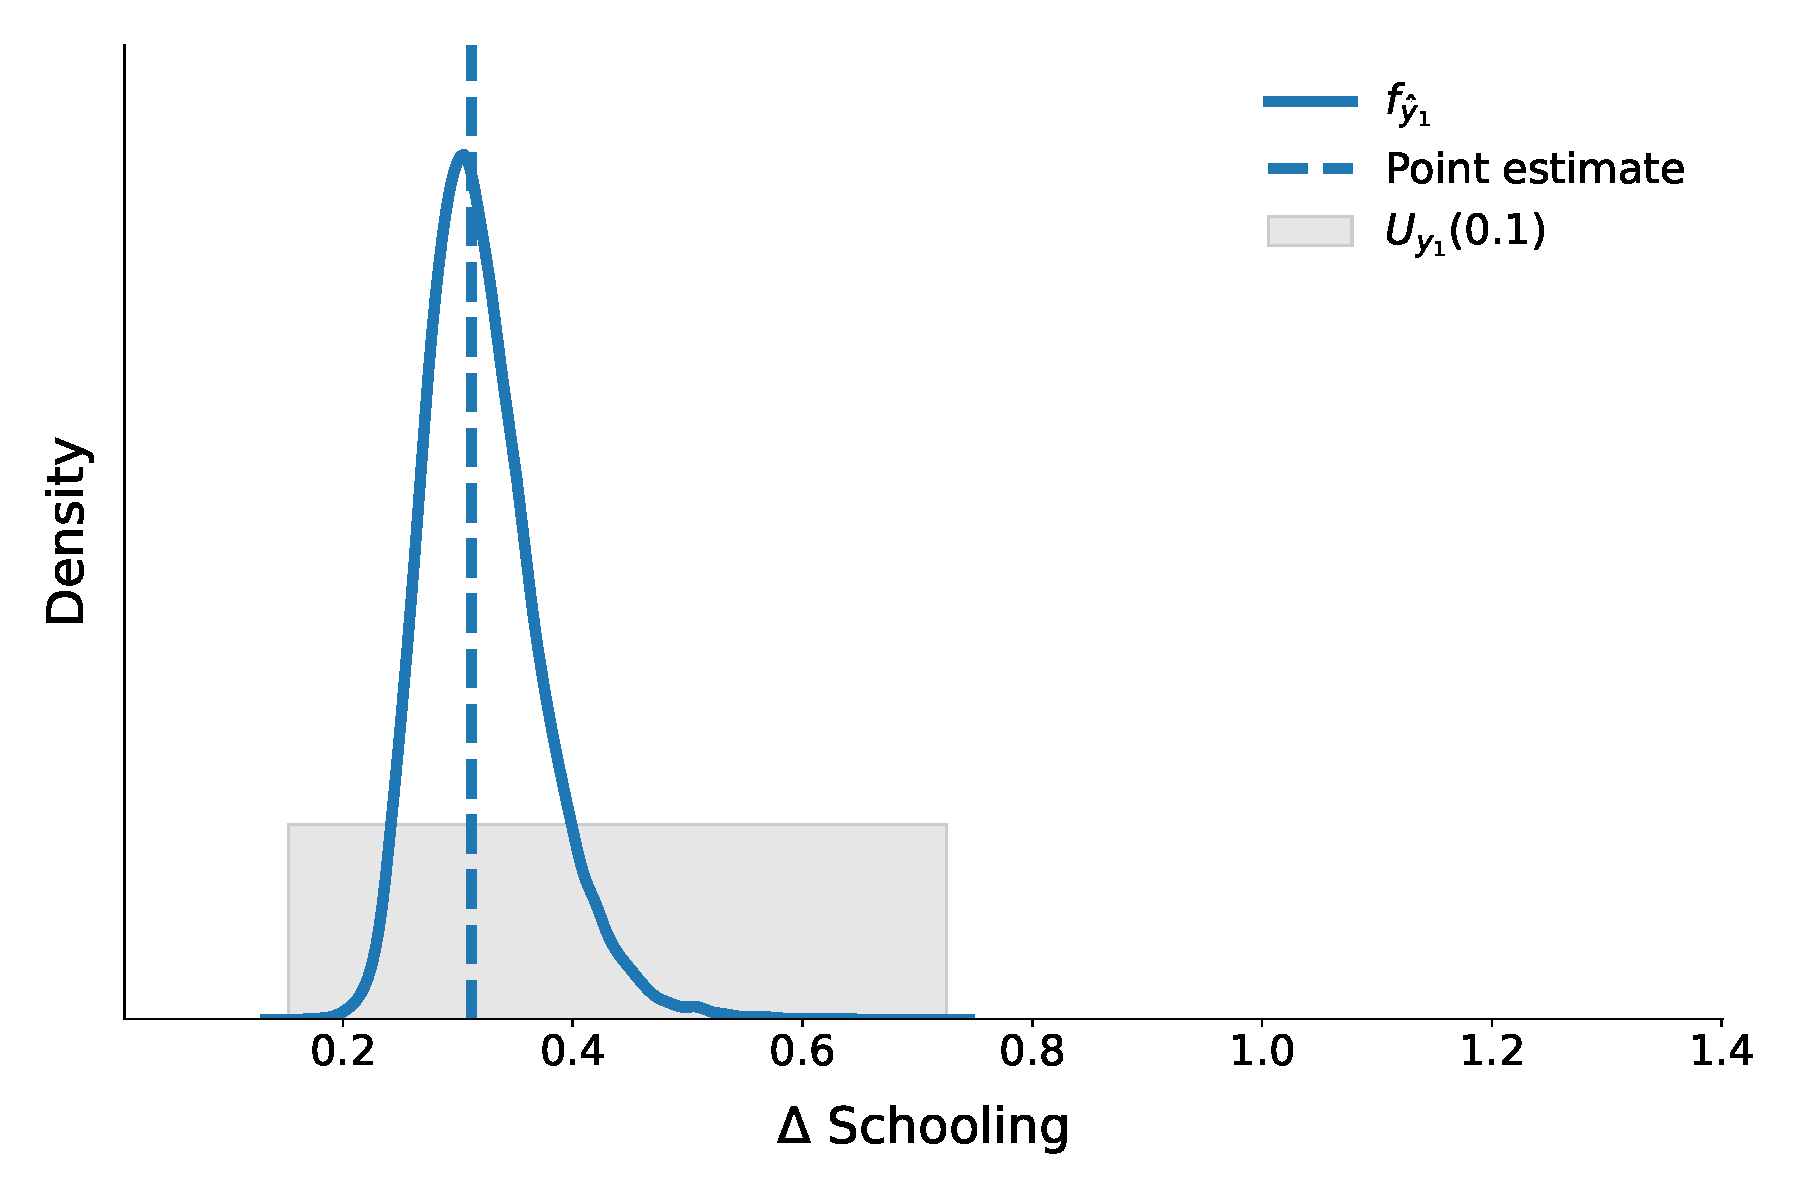
\includegraphics{fig-policy-average-years-type-0}}\label{type 0}}
    \subfloat[Type 2]{\scalebox{0.25}{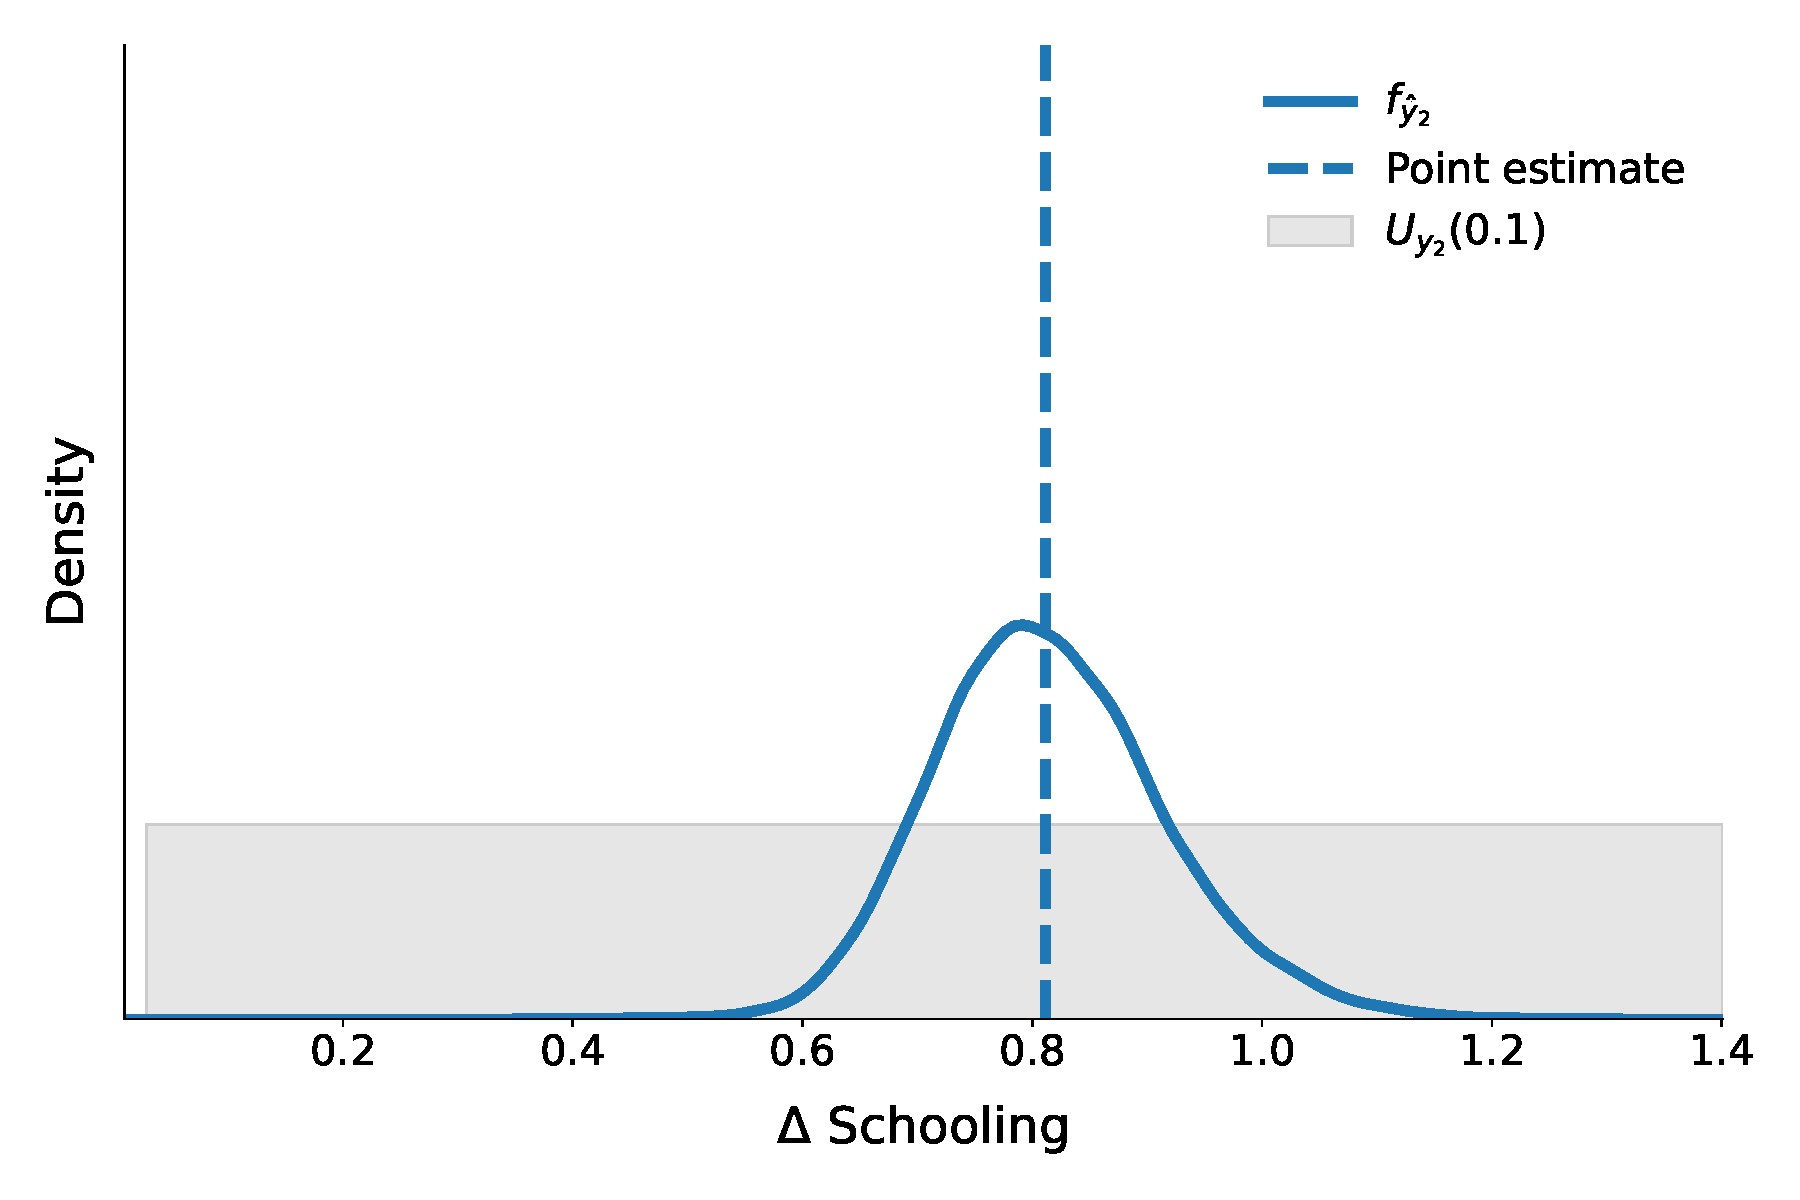
\includegraphics{fig-policy-average-years-type-1}}\label{type 2}}
    \caption{Prediction and uncertainty}
    \end{figure}
\end{frame}
%-------------------------------------------------------------------------------
%-------------------------------------------------------------------------------
\begin{frame}\label{fig:final-school}
    \begin{figure}[h!]\centering
    \subfloat[Type 3]{\scalebox{0.25}{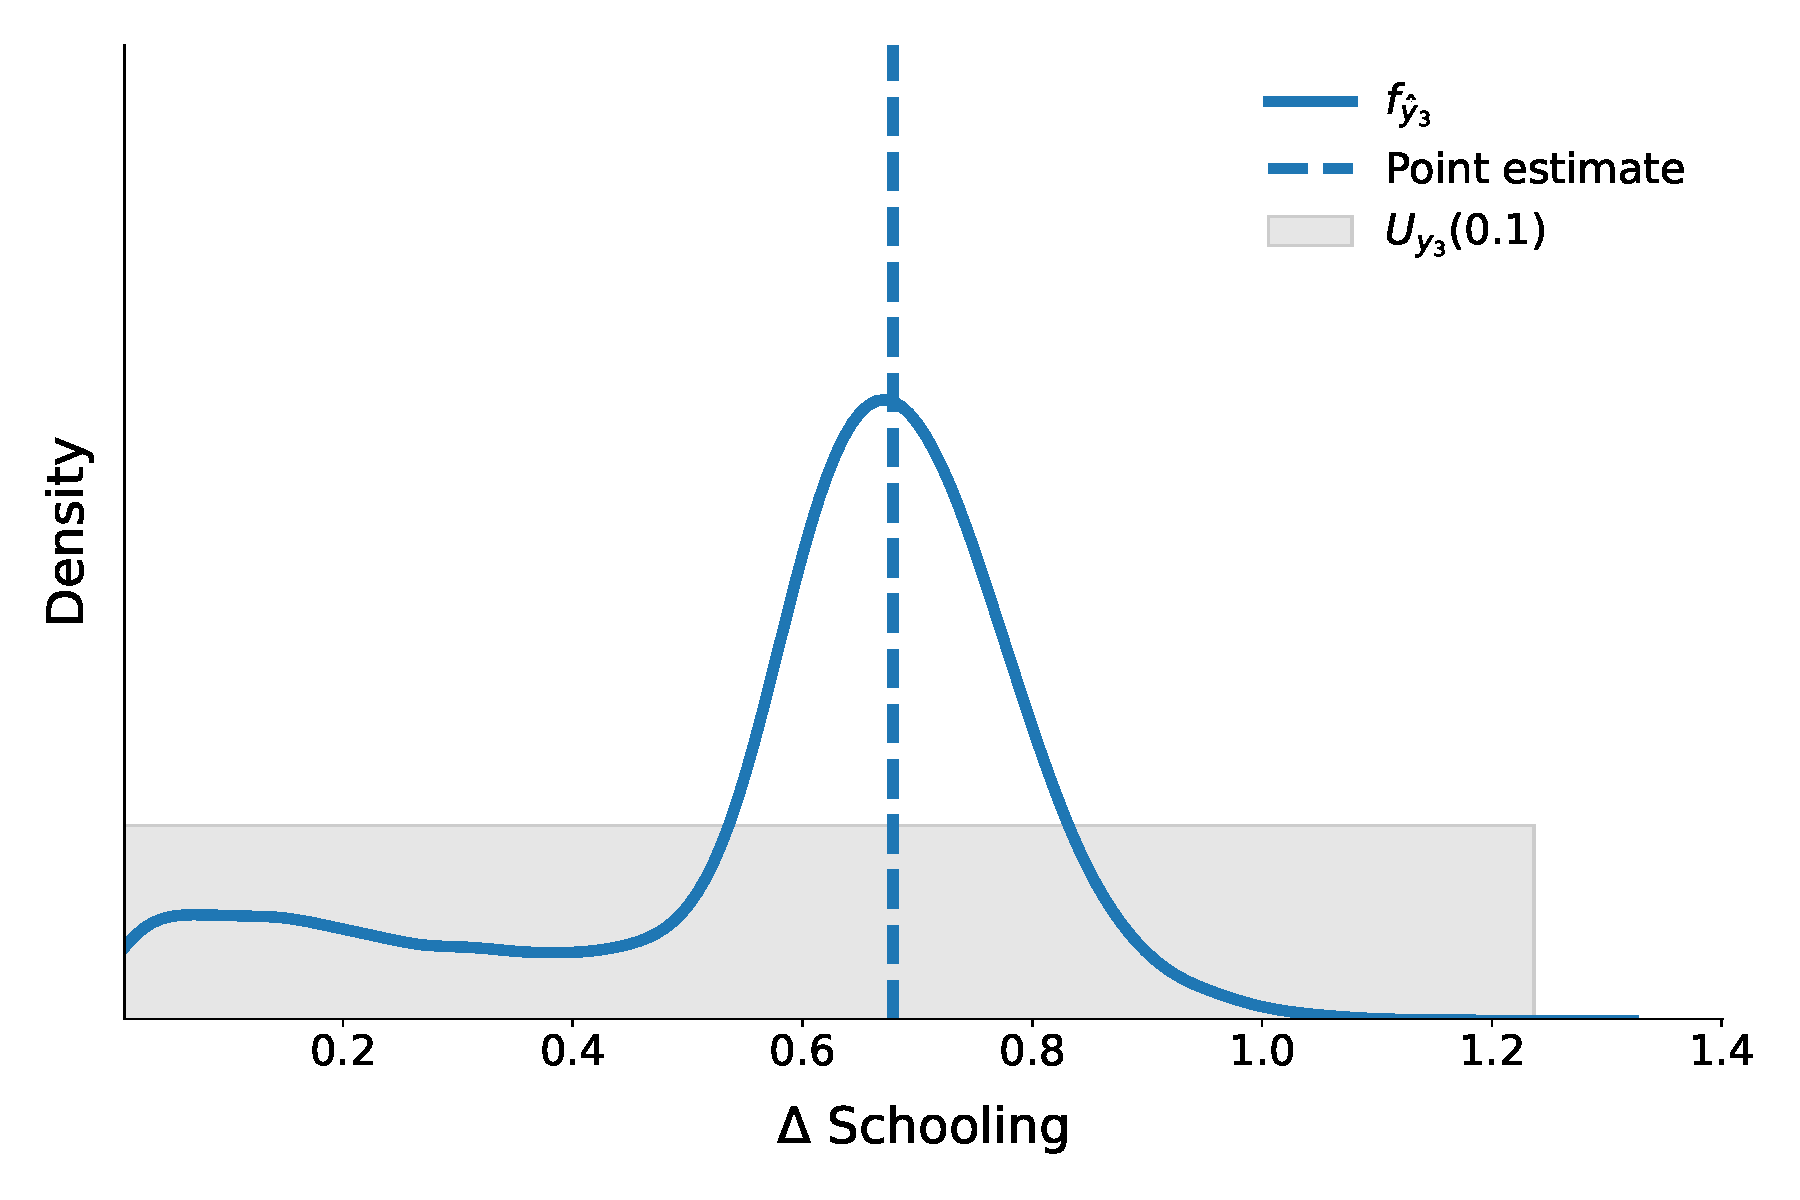
\includegraphics{fig-policy-average-years-type-2}}\label{type 0}}
    \subfloat[Type 4]{\scalebox{0.25}{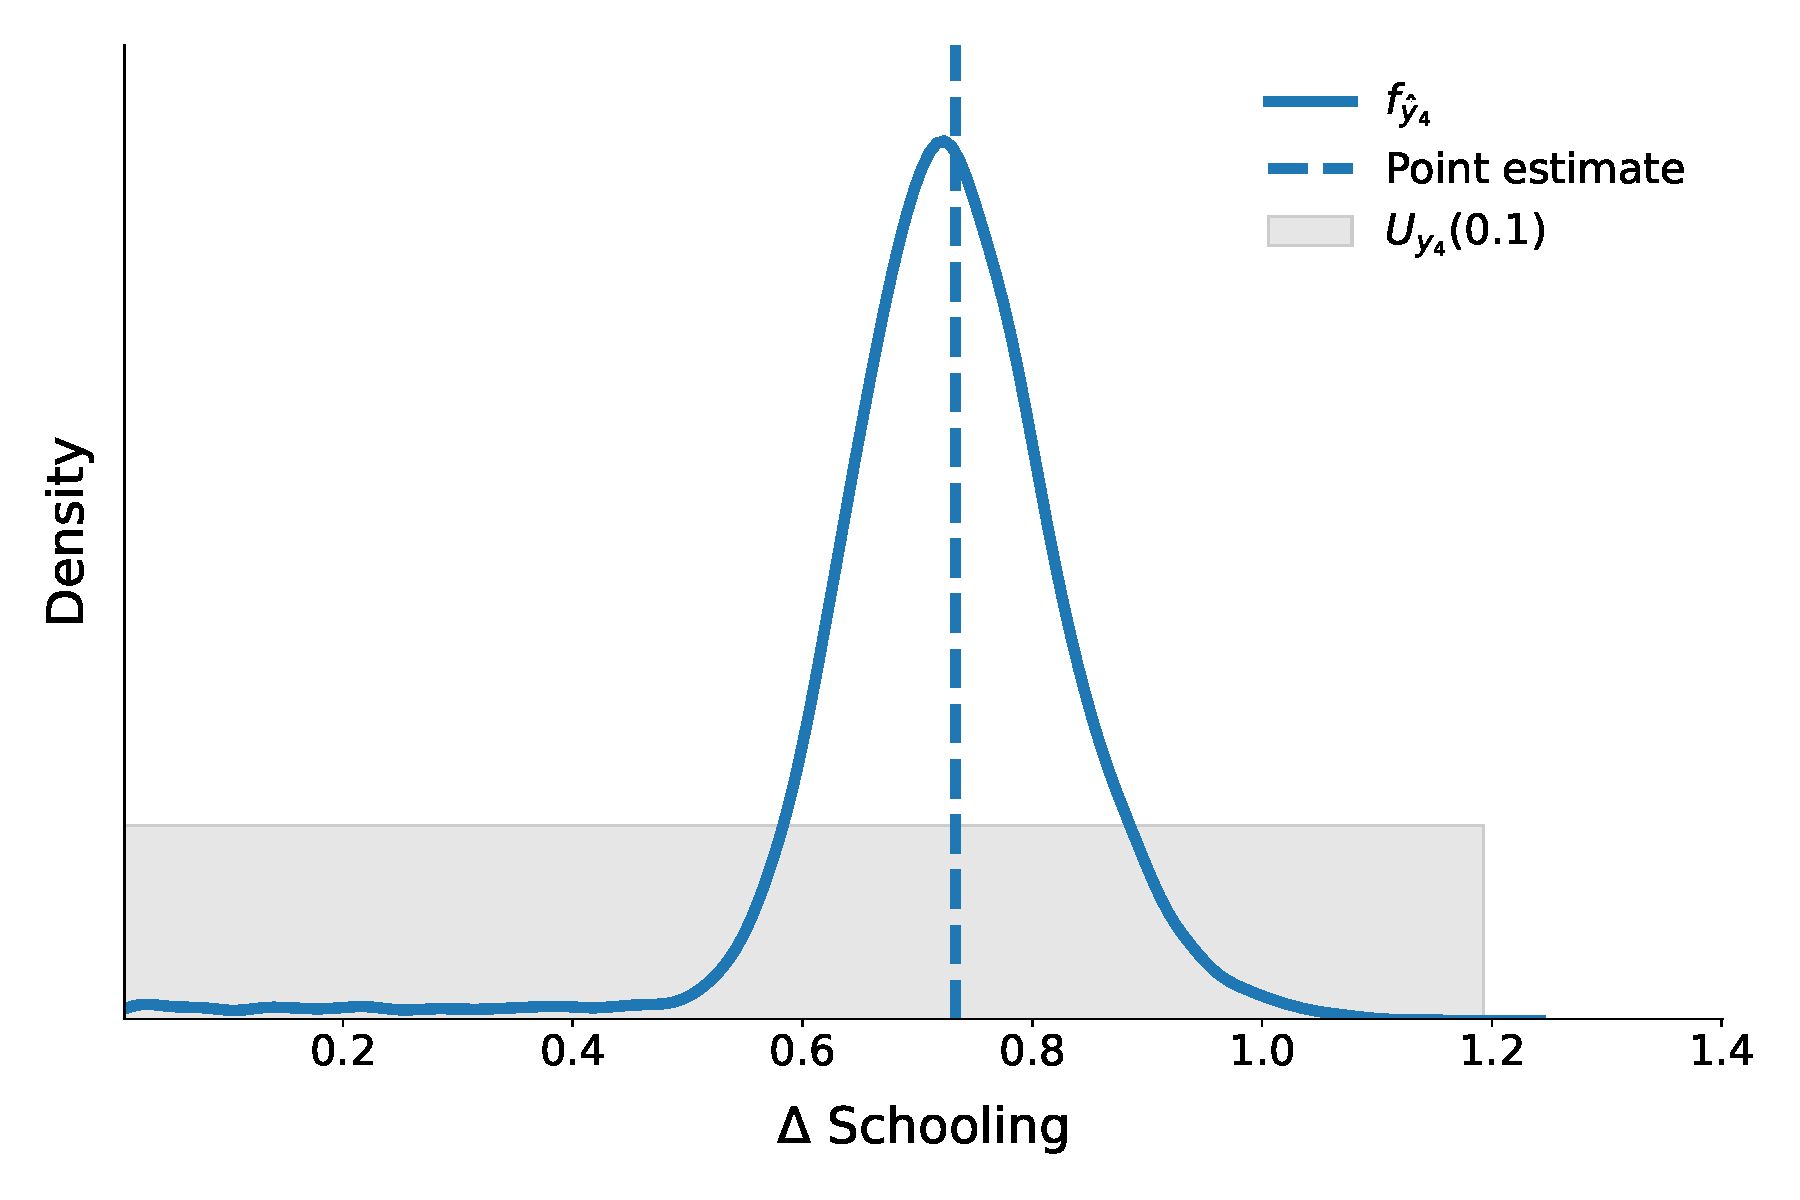
\includegraphics{fig-policy-average-years-type-3}}\label{type 2}}
    \caption{Prediction and uncertainty}
    \end{figure}
\end{frame}
%---------------------------------------------------------------------------------------------------
%---------------------------------------------------------------------------------------------------
\begin{frame}\frametitle{Examples of as-if analysis}\label{Examples of as-if analysis}
\vspace{0.3cm}\heading{Economic mechanisms}\vspace{0.3cm}
\begin{itemize}\setlength\itemsep{1em}
  \item \fullcite{Eisenhauer.2015b}
  \item \fullcite{Adda.2017}
  \item \fullcite{Blundell.2016}
\end{itemize}
\end{frame}
%---------------------------------------------------------------------------------------------------
%---------------------------------------------------------------------------------------------------
\begin{frame}\frametitle{Examples of as-if analysis}
\vspace{0.3cm}\heading{Optimal policy design}\vspace{0.3cm}
\begin{itemize}\setlength\itemsep{1em}
  \item \fullcite{Cunha.2010}
  \item \fullcite{Todd.2006}
  \item \fullcite{Blundell.2012}
\end{itemize}
\end{frame}
%---------------------------------------------------------------------------------------------------
%---------------------------------------------------------------------------------------------------
\begin{frame}{State of literature}
  \vspace{1cm}
  \begin{quote}\centering
    It is worth noting that no DCDP [discrete choice dynamic programming] work that we are aware of has ever reported a distribution of policy simulations that accounts for parameter uncertainty; and, it is also rarely done in nonstructural work.
  \end{quote}
  \centering
  \textendash \space \citet*{Keane.2011d}
\end{frame}
%---------------------------------------------------------------------------------------------------
%---------------------------------------------------------------------------------------------------
\begin{frame}{Confidence Set bootstrap algorithm}\vspace{0.5cm}\label{fig:algorithmic-description}

	\begin{algorithmic}\vspace{0.3cm}

    \For{$m = 1, \hdots, \bar{M}$}

    \State Draw $\btheta_m \sim \N(\hat{\btheta}, \hat{\bm{\Sigma}})$
    \State Compute $ c = (\btheta_m - \bar{\btheta} )^\prime \hat{\bm{\Sigma}}^{-1} (\btheta_m - \bar{\btheta})$

    \If{$(\hat{\btheta}_m - \hat{\btheta} )^\prime \hat{\bm{\Sigma}}^{-1} (\hat{\btheta}_m - \hat{\btheta}) \leq \chi_l^2(1 - \alpha)$}
    \State Compute $\hat{y}_{g,m} = \M_g(\hat{\btheta}_m )$
    \State Add $\hat{y}_{g,m}$ to sample $Y=\{\hat{y}_{g,1}, \hdots, \hat{y}_{g,m-1}\}$

  \EndIf

		\EndFor
    \State Set $\bTheta_{y_g}(\alpha) = [\min(Y), \max(Y)]$
		\vspace{0.3cm}
	\end{algorithmic}

  {\vspace{0.3cm} \hyperlink{determine-confidence-set}{\beamerbutton{Confidence set bootstrap}}}

\end{frame}
%---------------------------------------------------------------------------------------------------
%---------------------------------------------------------------------------------------------------
\begin{frame}{Model fit}\label{fig-model-fit}
  \begin{figure}[h!]\centering
  \subfloat[Average wage]{\scalebox{0.225}{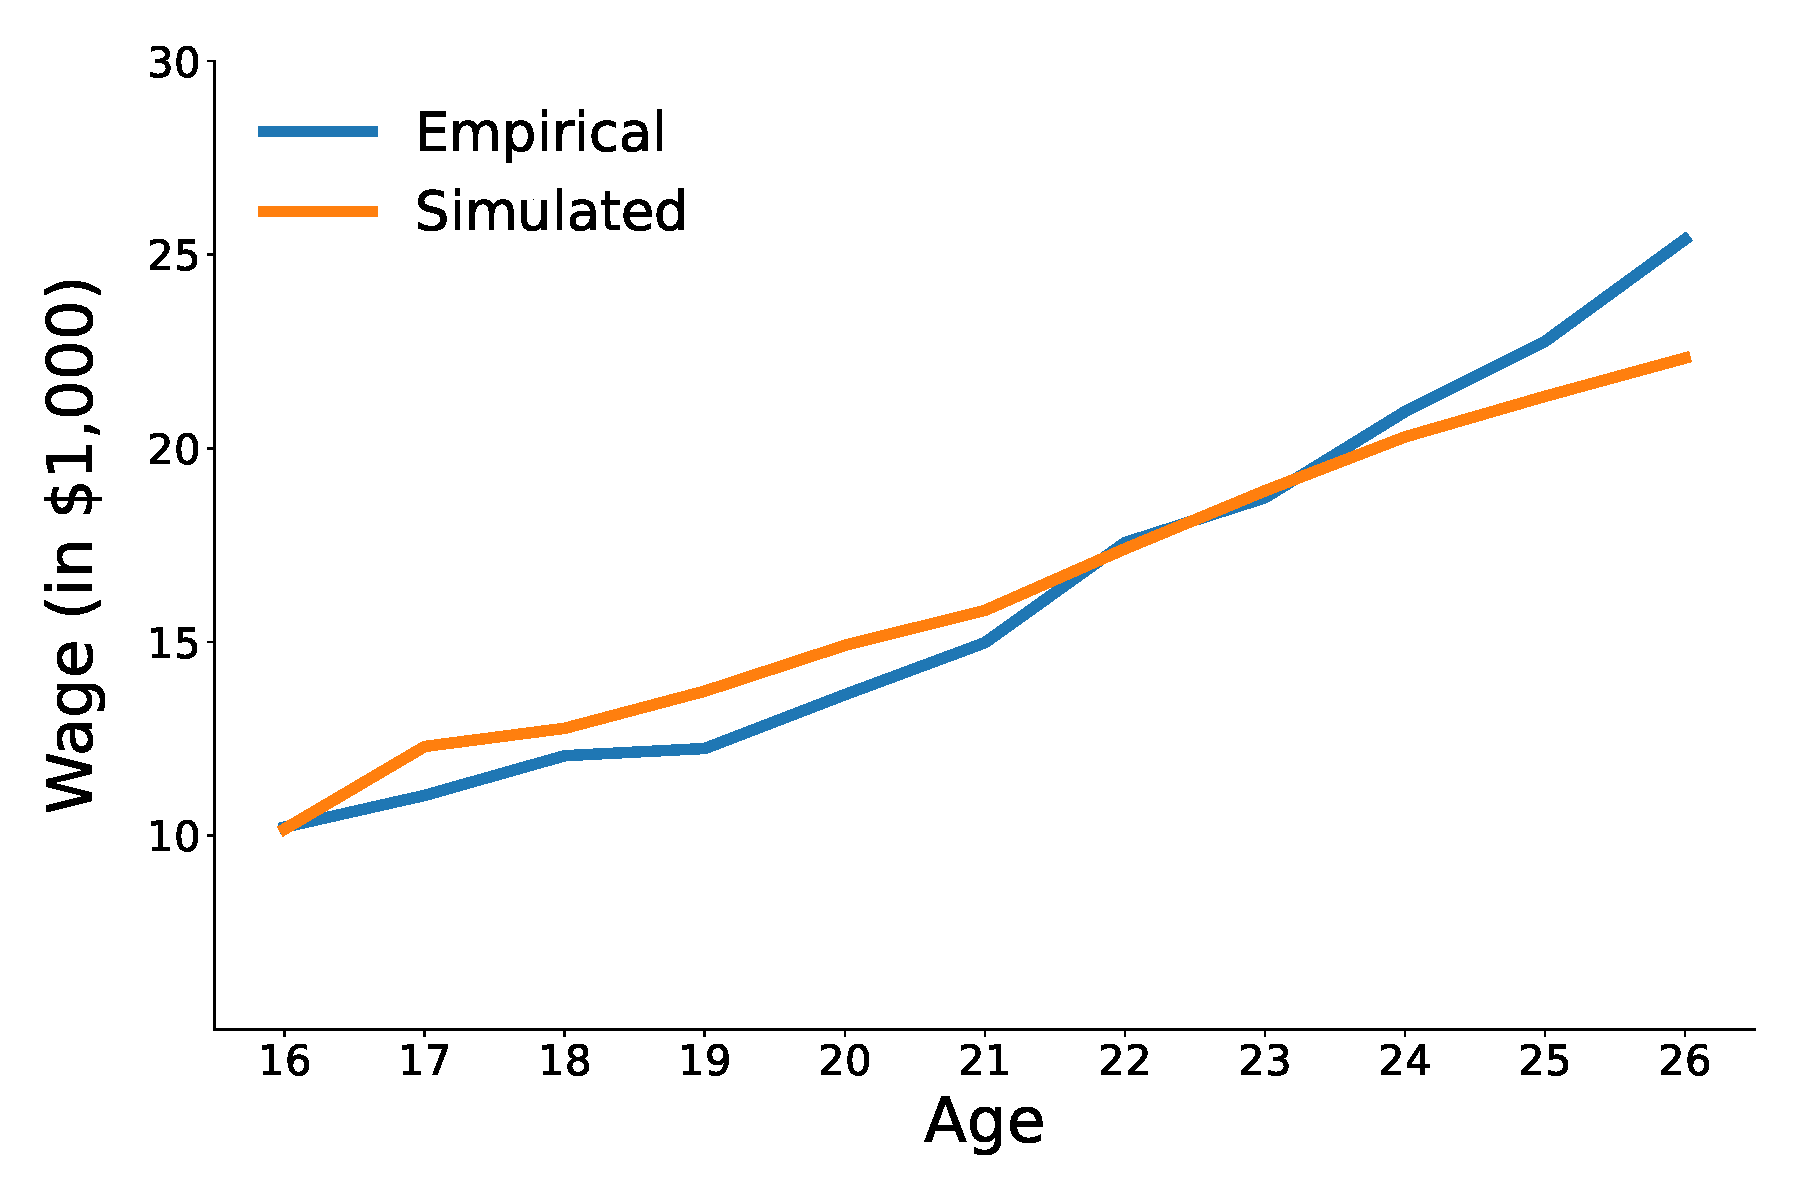
\includegraphics{fig-model-fit-wage-all}}}\hspace{0.5cm}
  \subfloat[Blue-collar]{\scalebox{0.225}{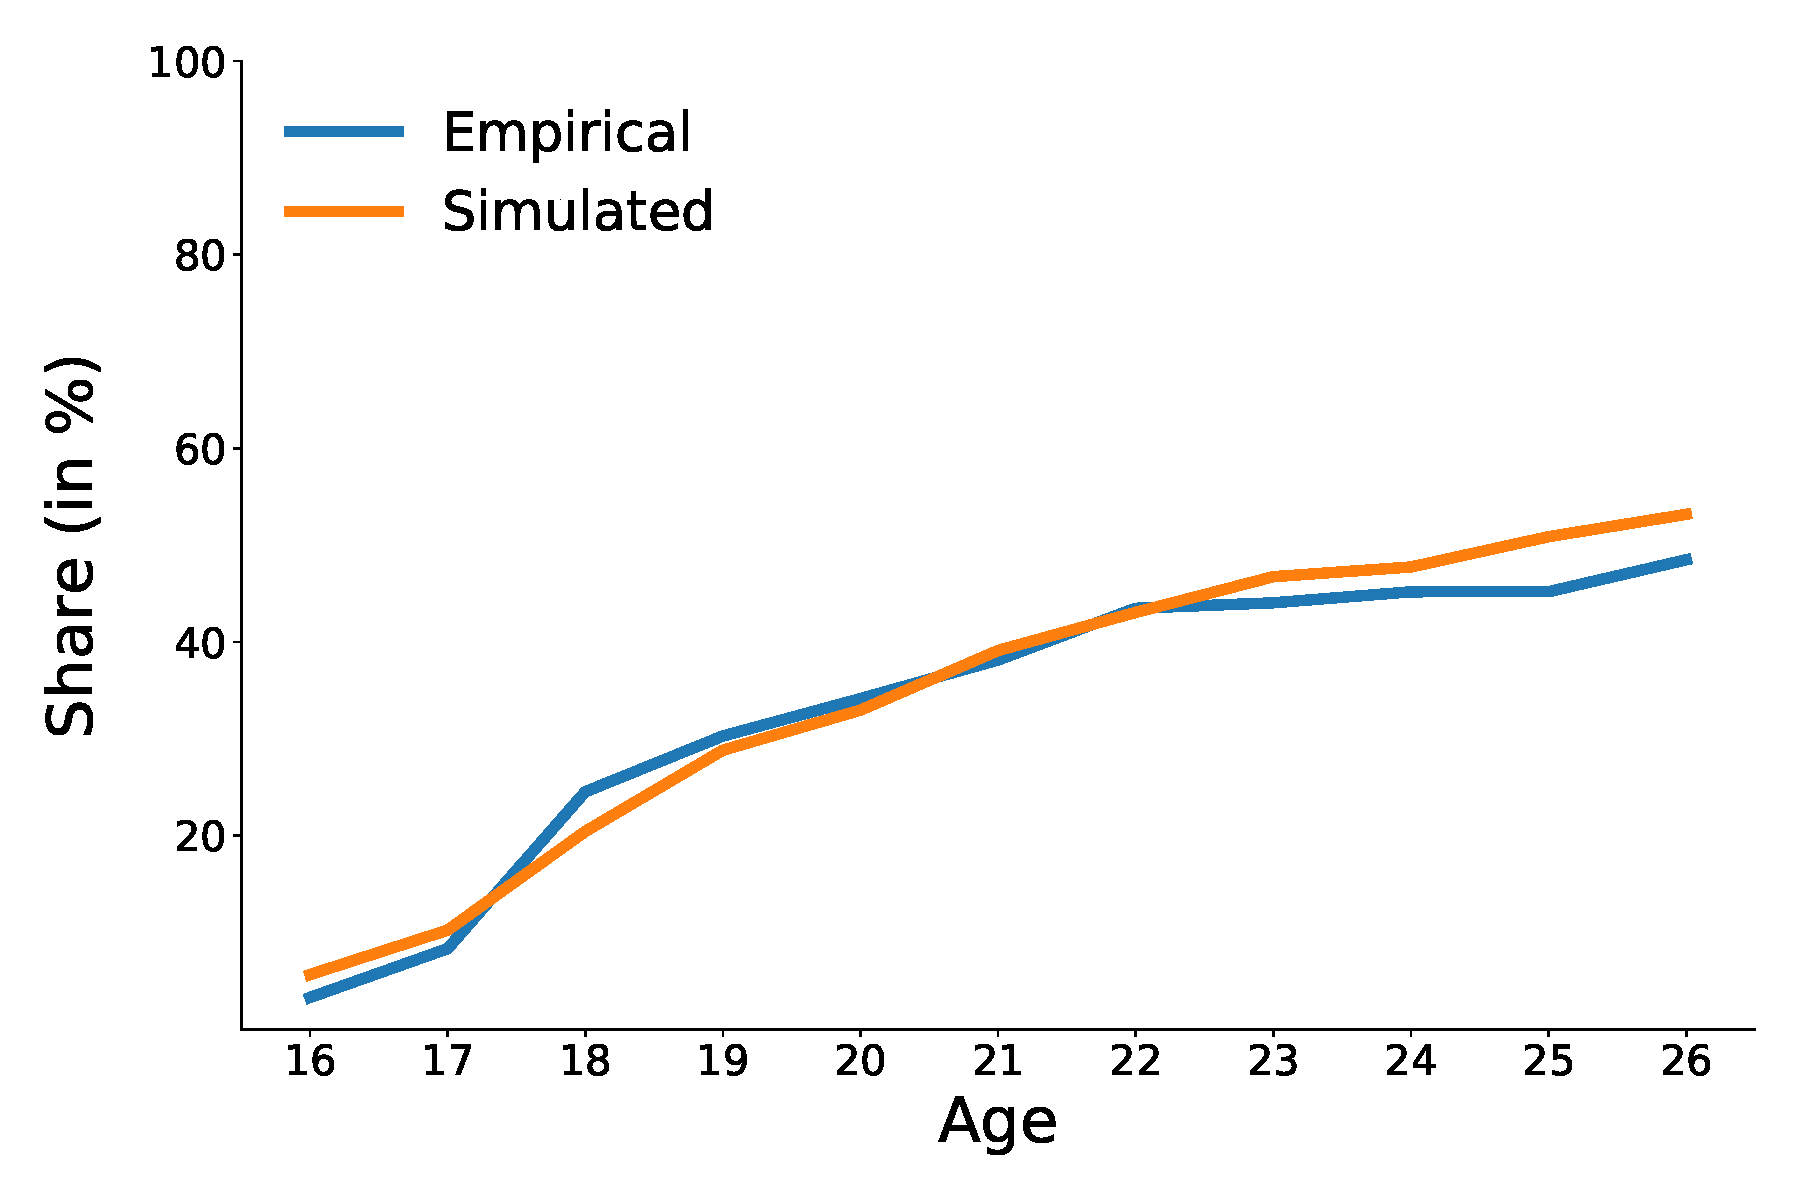
\includegraphics{fig-model-fit-choice-blue}}}
  \end{figure}
  \hyperlink{Data and estimation}{\beamerbutton{Data and estimation}}

\end{frame}
%---------------------------------------------------------------------------------------------------
%---------------------------------------------------------------------------------------------------
\begin{frame}{Uncertainty propagation}
  \begin{figure}[h!]\centering
  \scalebox{0.3}{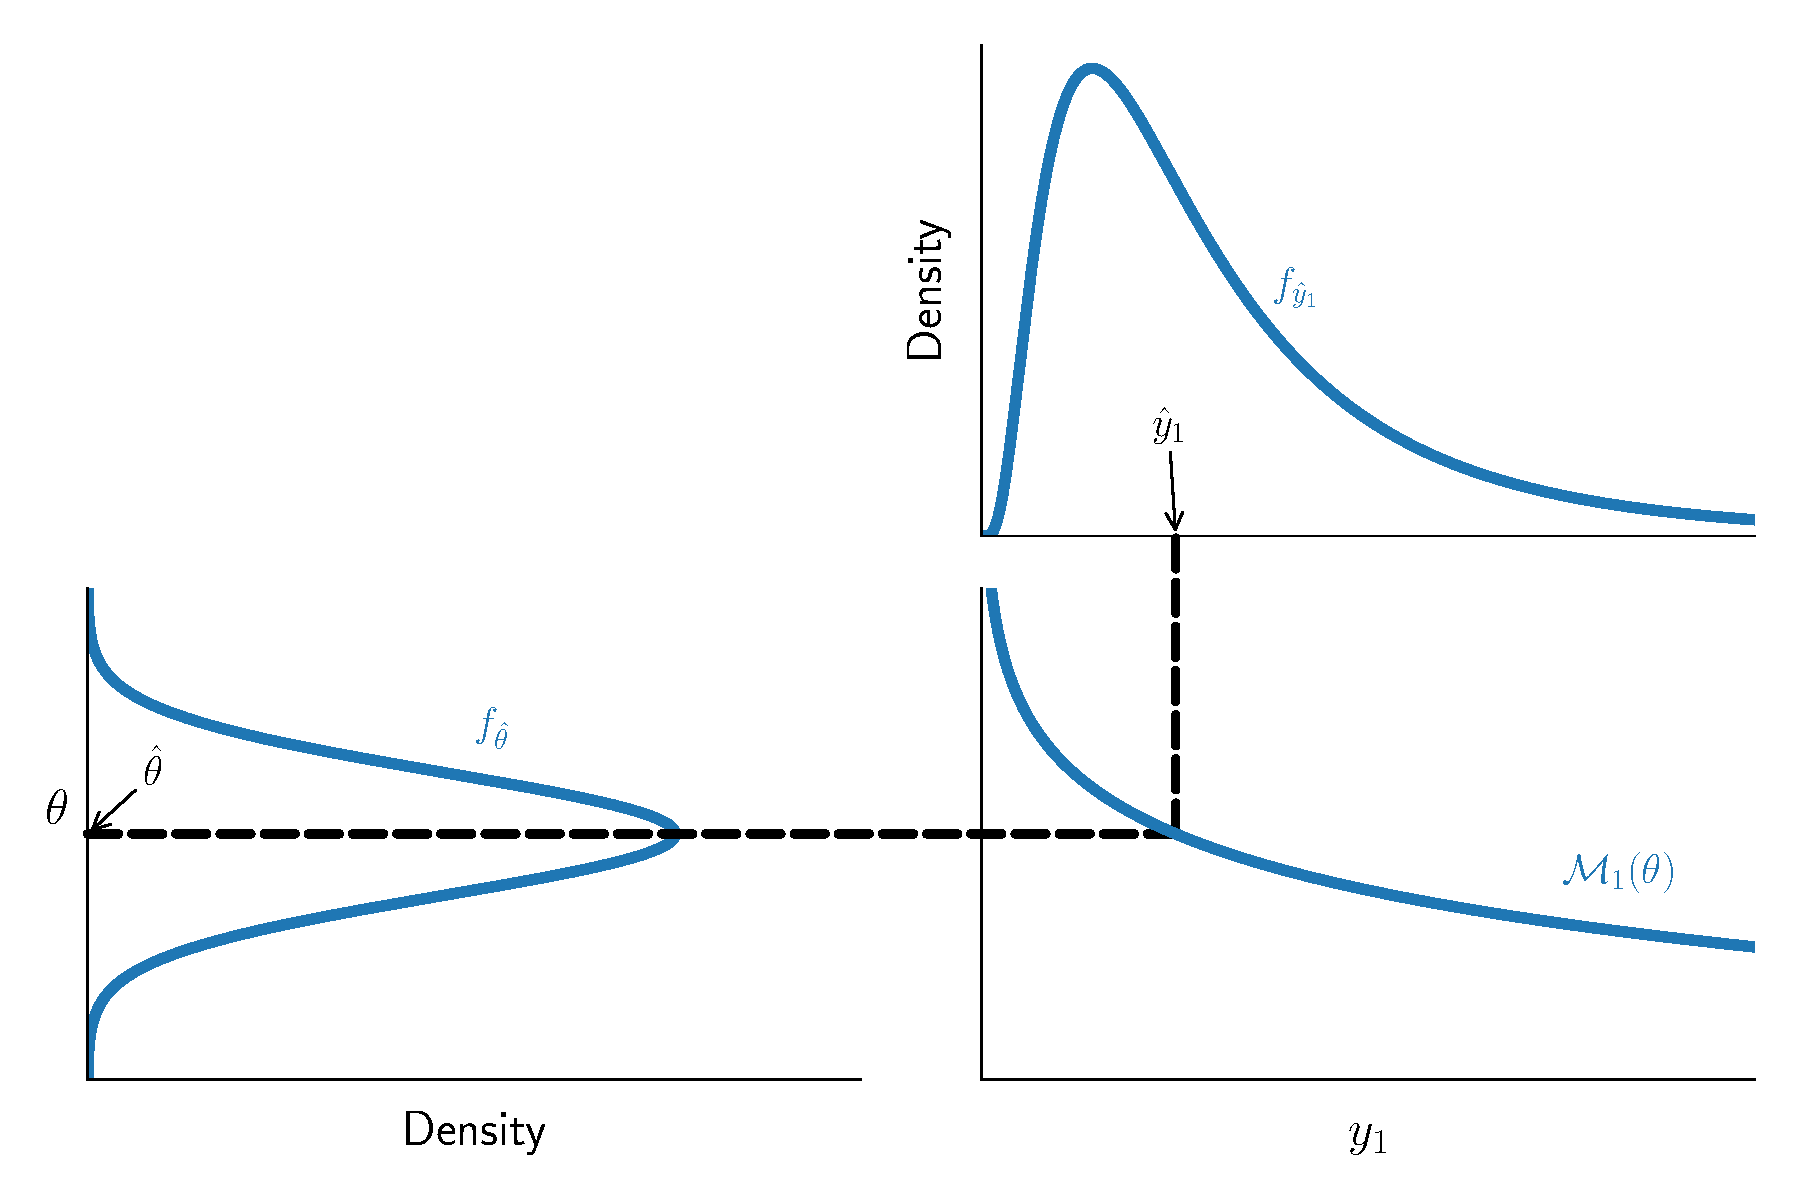
\includegraphics{fig-illustration-transformation.pdf}}
  \end{figure}
\end{frame}
%---------------------------------------------------------------------------------------------------
%---------------------------------------------------------------------------------------------------
\begin{frame}{Tracing out the impact of time preference}\vspace{0.3cm}
  \begin{figure}[h!]\centering
  \scalebox{0.275}{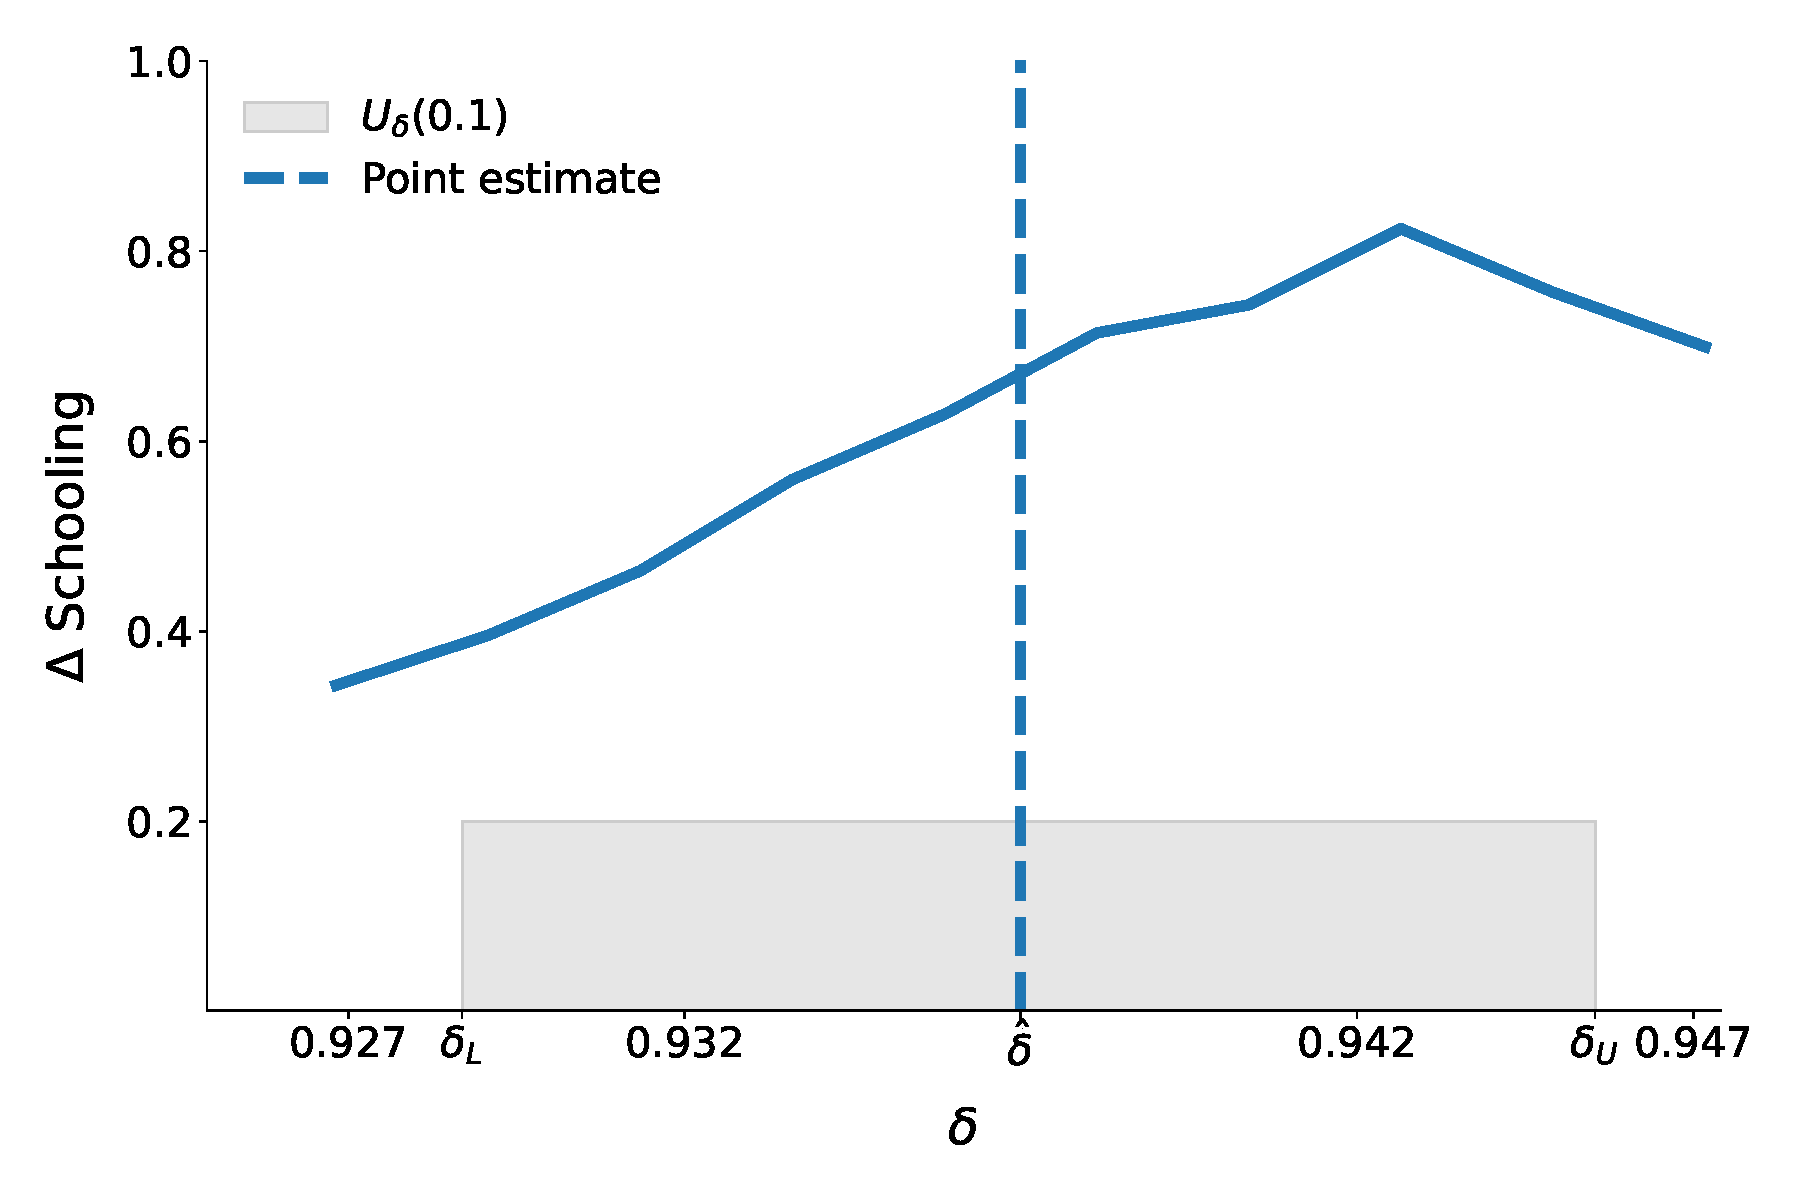
\includegraphics{fig-trace-delta}}
\end{figure}\vspace{-0.5cm}
  \hyperlink{fig:final-school-policy}{\beamerbutton{Explore the economics behind it}}
\end{frame}
%---------------------------------------------------------------------------------------------------
%---------------------------------------------------------------------------------------------------
\begin{frame}\frametitle{Community code}

\vspace{0.3cm}\textbf{\raisebox{-0.04cm}{
\includegraphics[height=0.60cm]{crop-respy-logo-bare.pdf}}\hspace{0.05cm} {\Large respy}}\vspace{0.50cm}

A research code for the flexible specification, simulation, and estimation of Eckstein--Keane--Wolpin models.\\
\vspace{0.45cm}

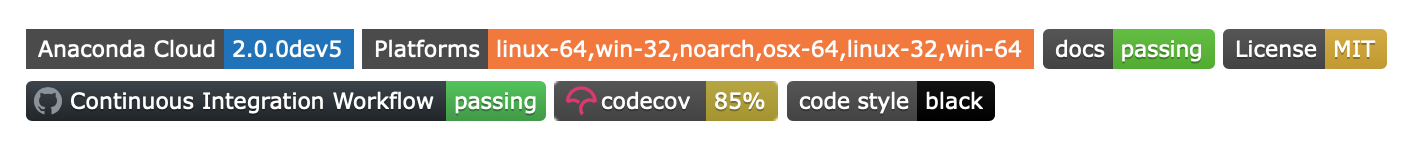
\includegraphics[width=0.9\textwidth]{crop-respy-engineering.png}\\
\vspace{0.50cm}

\hspace{-0.2cm}\begin{tabular}{ll}
\textbf{Core devs} & Tobias Raabe, Janoś Gabler\\
\textbf{Docs}      & \url{respy.readthedocs.io}
\end{tabular}

\end{frame}
%---------------------------------------------------------------------------------------------------
%---------------------------------------------------------------------------------------------------
\begin{frame}{Sample size}
  \begin{figure}
  \scalebox{0.30}{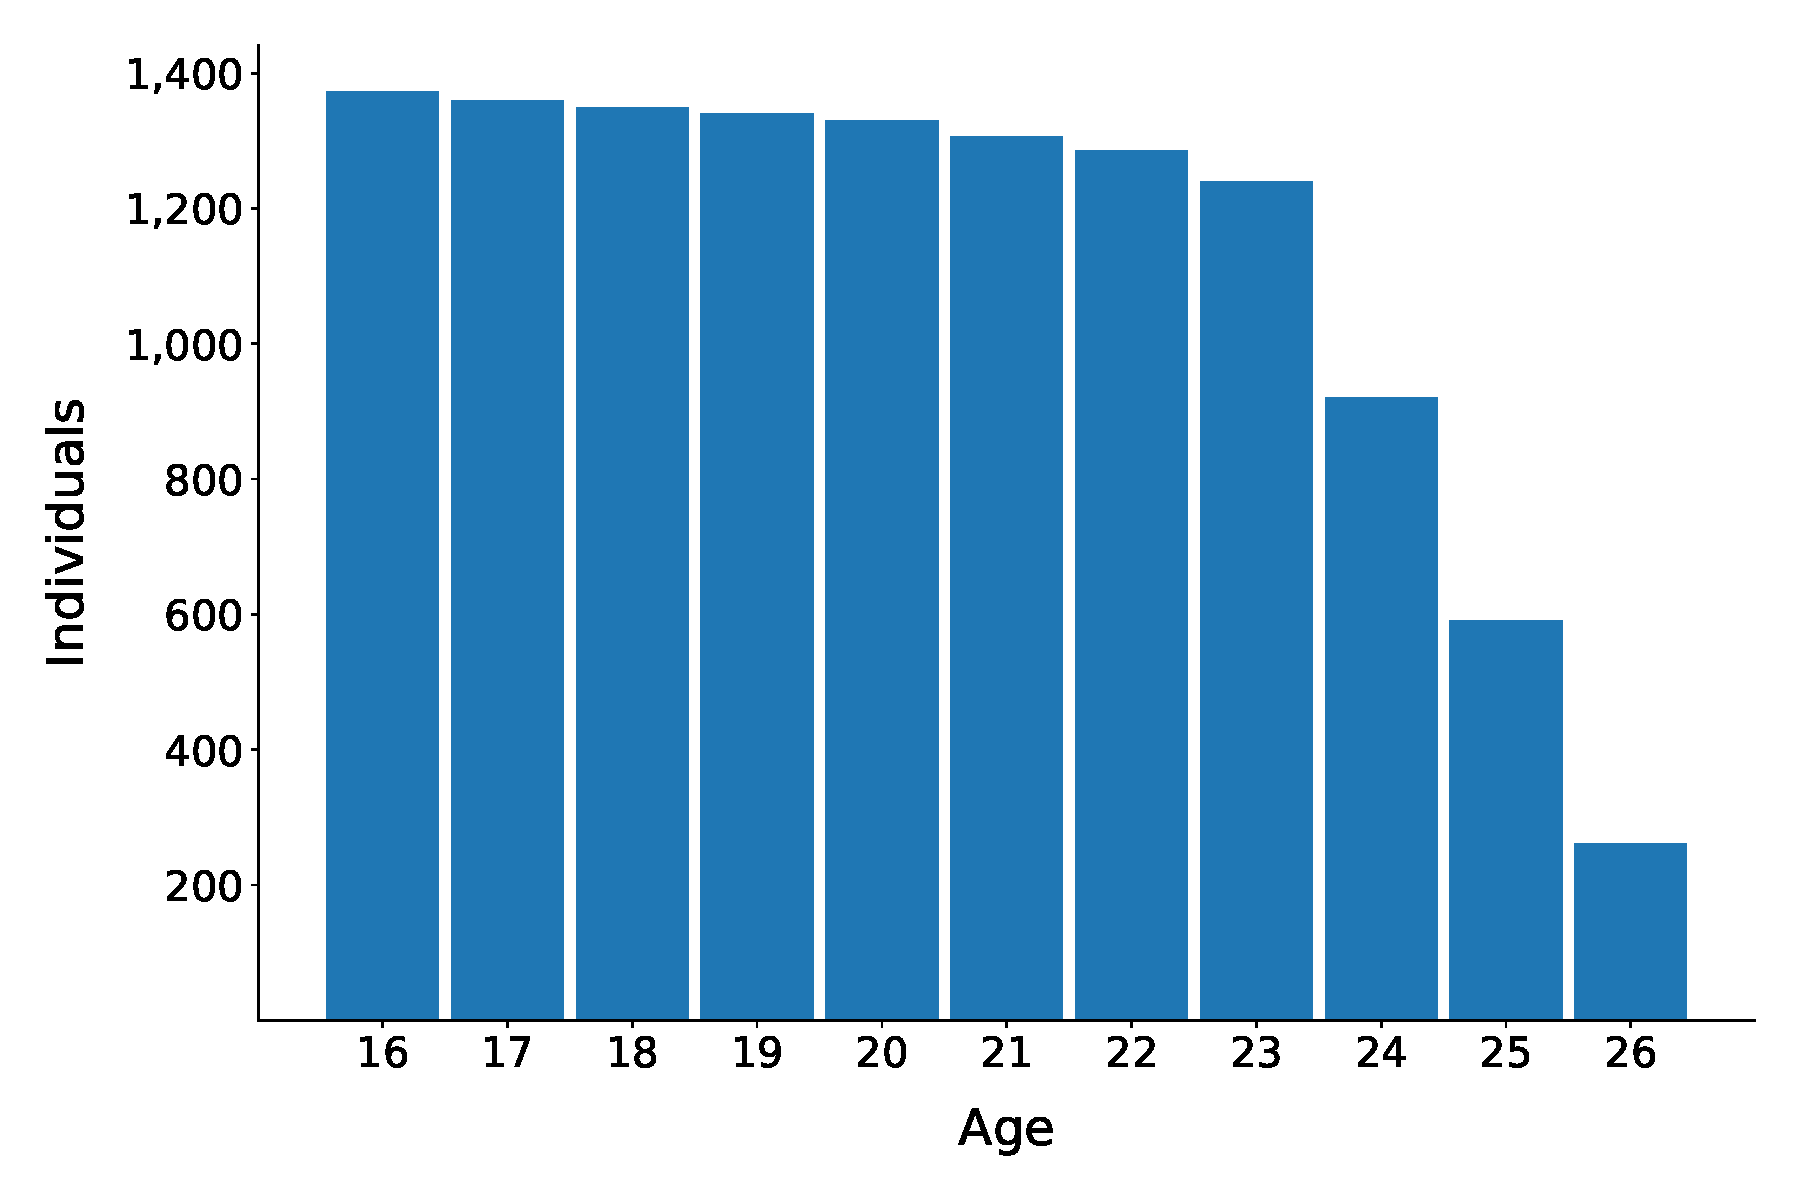
\includegraphics{fig-sample-size}}
  \end{figure}
\end{frame}
%---------------------------------------------------------------------------------------------------
%---------------------------------------------------------------------------------------------------
\begin{frame}{Related literature}\vspace{0.3cm}
  	\begin{itemize}\setlength\itemsep{1em}
  	\item \textbf{Local sensitivity analysis:} \citet{Andrews.2017}, \citet{Andrews.2020}, \citet{Christensen.2019}, \citet{Jorgensen.2021}
    \item \textbf{Global sensitivity analysis:} \citet{Cai.2019}, \citet{Harenberg.2019}, \citet{Miftakhova.2021}
    \item \textbf{Public policy and uncertainty:} \citet{Berger.2021}, \citet{Hansen.2021}, \citet{Manski.2013}
    \item \textbf{Statistical decision theory:} \citet{Gilboa.2009}, \citet{Manski.2021}

  	\end{itemize}
\end{frame}
%---------------------------------------------------------------------------------------------------
%---------------------------------------------------------------------------------------------------
\begin{frame}\frametitle{Next steps}\vspace{0.3cm}

\begin{itemize}\setlength\itemsep{1em}
  \item Generalize our work building on asymptotic optimality theory for statistical treatment rules
  \item Address the computational burden of our analysis using surrogate modeling and adaptive sampling methods
  \item Incorporate ideas from the literature on global sensitivity analysis to identify the parameters most responsible for the uncertainty in predictions
  \item Link our work with the literature on inference under (local) model misspecification to refine the construction of our uncertainty sets
\end{itemize}
\end{frame}
%---------------------------------------------------------------------------------------------------
%---------------------------------------------------------------------------------------------------
\backupend
